%# -*- coding: utf-8-unix -*-
%%==================================================
%% thesis.tex
%%==================================================

% 双面打印
%\documentclass[doctor, openright, twoside]{sjtuthesis}
\documentclass[bachelor, openany, oneside, english, submit]{sjtuthesis}

% \documentclass[master, review]{sjtuthesis}
% \documentclass[%
%   bachelor|master|doctor,	% 必选项
%   fontset=fandol|windows|mac|ubuntu|adobe|founder, % 字体选项
%   oneside|twoside,		% 单面打印,双面打印(奇偶页交换页边距,默认)
%   openany|openright, 		% 可以在奇数或者偶数页开新章|只在奇数页开新章(默认)
%   english,			% 启用英文模版
%   review,	 		% 盲审论文,隐去作者姓名、学号、导师姓名、致谢、发表论文和参与的项目
%   submit			% 定稿提交的论文,插入签名扫描版的原创性声明、授权声明 
% ]

% 逐个导入参考文献数据库
\addbibresource{bib/thesis.bib}
% \addbibresource{bib/chap2.bib}

\begin{document}

%% 无编号内容:中英文论文封面、授权页
%# -*- coding: utf-8-unix -*-
\title{深度学习中高校高效学习新样本}
\author{宋肇哲}
\advisor{卢策吾}
% \coadvisor{某某教授}
\defenddate{2014年12月17日}
\school{上海交通大学}
\institute{电子信息与电气工程学院}
\studentnumber{5140309514}
\major{电子信息科学类}

\englishtitle{Efficient Methods for Incremental Learning in Deep Neural Networks}
\englishauthor{\textsc{Zhaozhe Song}}
\englishadvisor{Prof. \textsc{Cewu Lu}}
% \englishcoadvisor{Prof. \textsc{Uom Uom}}
\englishschool{Shanghai Jiao Tong University}
\englishinstitute{\textsc{Depart of XXX, School of XXX} \\
  \textsc{Shanghai Jiao Tong University} \\
  \textsc{Shanghai, P.R.China}}
\englishmajor{A Very Important Major}
\englishdate{Dec. 17th, 2014}


\maketitle

\makeatletter
\ifsjtu@submit\relax
	\includepdf{pdf/original.pdf}
	\cleardoublepage
	\includepdf{pdf/authorization.pdf}
	\cleardoublepage
\else
\ifsjtu@review\relax
% exclude the original claim and authorization
\else
	\makeDeclareOriginal
	\makeDeclareAuthorization
\fi
\fi
\makeatother


\frontmatter 	% 使用罗马数字对前言编号

%% 摘要
\pagestyle{main}
%# -*- coding: utf-8-unix -*-
%%==================================================
%% abstract.tex for SJTU Master Thesis
%%==================================================

\begin{abstract}

在深度学习系统中,数据往往是一步步地采集和增加的。在深度学习领域,一个重要而困难的问题是开发出一套能随着数据的增加而不断提升自己知识的系统。在以往的文献中,这个问题通常被称作增量学习。这样的系统,需要不断地快速地在已有的模型中融合进去新的知识,而不是每次增加了新数据都重新把内部的深度神经网络重新训练一遍,否则开销会很大。在这个工作中,我们利用在物体检测领域经常使用的困难负样本挖掘的方法,提出了一套针对类别不断增加时的增量学习算法。在每次新的类别到来的时候,我们的算法的主循环可以大致分解为以下两步:1)用所数据数据继续训练深度神经网络,并且记录下每个旧类别对神经网络来说最困难的一个图片集合。2)在最困难的图片集合中采样,用它们和新类别的数据再次训练当前的深度神经网络。在第一步中,神经网络模型可以对真实的数据分布进行学习。在第二步中,因为有大量新样本比例,模型被迫快速地学习出新样本的特征,同时又不忘记旧类别中最困难的那些样本,如此往复。我们使用几个典型的深度学习网络结构在图像分类数据集CIFAR-10和CIFAR-100上进行了充分的实验证明我们算法的有效性。我们的方法不仅让模型能快速学习出关于新样本的知识,还能对旧样本维持一个很高的准确率。我们用实验说明我们方法可以始终维持一个较高的平均准确率,而其他底线方法或其他论文中的策略都会让模型很快失败。在CIFAR-100数据集上,我们的算法相比重新训练网络能节省40倍的时间,而仅有$2\%$左右的准确率损失。我们的实验也表明我们的模却是确实可以逐渐学习出越来越好的特征来识别逐渐增长的类别。


\keywords{\large 深度学习 \quad 增量学习 \quad 困难负样本挖掘 \quad 图像分类}
\end{abstract}

\begin{englishabstract}

In deep learning systems, data is usually collected incrementally. A major and tough problem in the field of deep learning is the development of systems that learns incrementally over time from a stream of available data. This problem is typically called incremental learning in literature. Such systems should continuously incorporate new knowledge in a quick manner, without having to re-train the inherent deep neural network every time from scratch. In this work, we proposed an algorithm for class-incremental learning systems, by utilizing hard negative mining techniques that were popular in recent object detection pipelines. Upon the addition of a new class, our main algorithm can be broken down into two steps that are iterated for several times: 1) Further train the deep neural network with all data, and record the hardest examples from every learned class. 2) Sample the hardest images that the model has already learned, and use them, together with the new class of data, to further train the neural network. In the first step, the model learns the data in a true distribution. In the second step, since the majority are new examples, the model is forced to learn features quickly for the new class, but also not forgetting the hardest old examples. We conducted thorough experiments on the image classification datasets CIFAR-10 and CIFAR-100 using representative deep learning structures, and proved the effectiveness of our method. Our method not only enables the model to learn knowledge on the new class very quickly, but is also capable of maintaining high accuracy on the old classes. Our algorithm keeps a high average accuracy our time, while baseline strategies or strategies from other papers fail quickly. In CIFAR-100, our algorithm saves $40\times$ time compared to re-training from scratch when a new class of training images are added, with only about $2\%$ average accuracy loss. Experiments also indicate that our model indeed gradually learns better features to correctly classify more objects. 

\englishkeywords{\large deep learning, incremental learning, hard negative mining, image classification}
\end{englishabstract}



%% 目录、插图目录、表格目录
\tableofcontents
\listoffigures
\addcontentsline{toc}{chapter}{\listfigurename} %将插图目录加入全文目录
\listoftables
\addcontentsline{toc}{chapter}{\listtablename}  %将表格目录加入全文目录
\listofalgorithms
\addcontentsline{toc}{chapter}{\listalgorithmname} %将算法目录加入全文目录

%%# -*- coding: utf-8-unix -*-
\begin{nomenclaturename}
\label{chap:symb}

\begin{longtable}{rl}
$\epsilon$     & 介电常数 \\
 $\mu$ 		& 磁导率 \\

\end{longtable}

\end{nomenclaturename}
 % 主要符号、缩略词对照表

\mainmatter	% 使用阿拉伯数字对正文编号

%% 正文内容
\pagestyle{main}
%# -*- coding: utf-8-unix -*-
%%==================================================
%% chapter01.tex for SJTU Master Thesis
%%==================================================

%\bibliographystyle{sjtu2}%[此处用于每章都生产参考文献]
\chapter{Introduction}
\label{chap:intro}
\section{Motivation and Contribution}
In many real world applications, data is collected incrementally. For example, the large-scale image classification dataset ImageNet is becoming larger and larger when more notations become available. For another practical example and also the main origination of this project, imagine a commercial system that can classify merchandise correctly based on the image of the merchandise, as illustrated in Fig.~\ref{fig:merchandise}. It has a large potential to be used by automatic robotic arms used in automatic logistics center or autonomous supermarkets. A robotic arm is shown in Fig.~\ref{fig:arm}. Since there will always be new types of merchandise emerging, this system should always adapt to new merchandise types but also not forgetting the learned merchandise types. Thus in this example, the merchandise data is also incremental.

\begin{figure}[!htp]
	\centering
	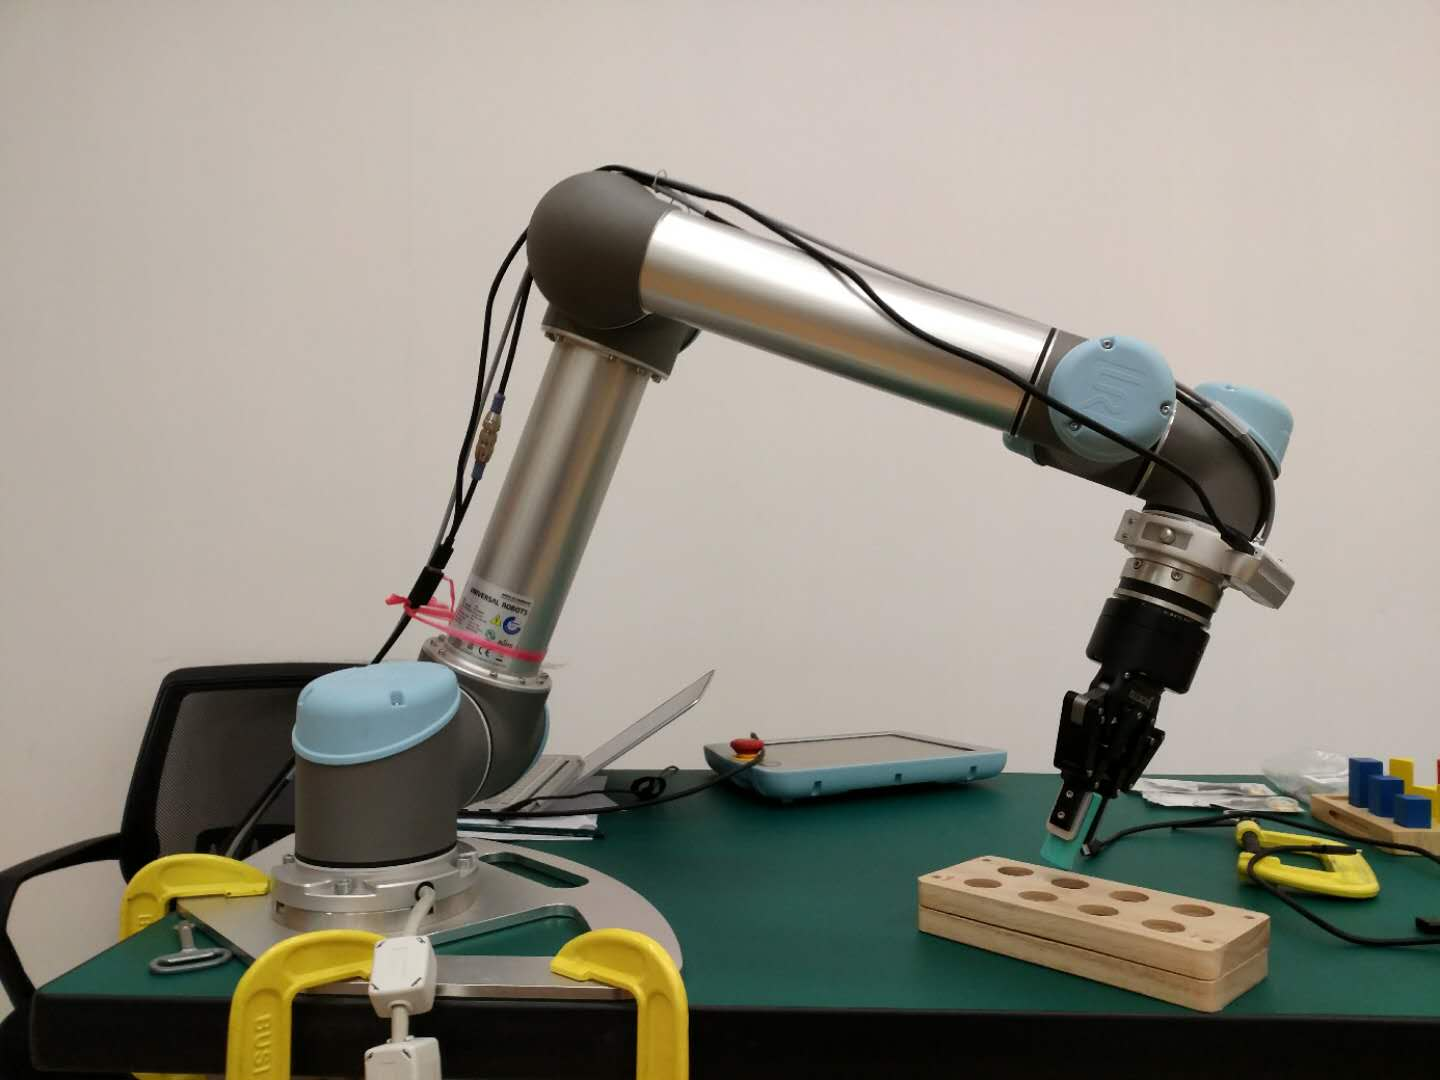
\includegraphics[width=14cm]{arm.jpg}
	\bicaption[Example of a robotic arm for autonomous logistics center]
	{可用于物流系统的机械臂示意图}
	{Example of a robotic arm for autonomous logistics center}
	\label{fig:arm}
\end{figure}
\begin{figure}[!htp]
	\centering
	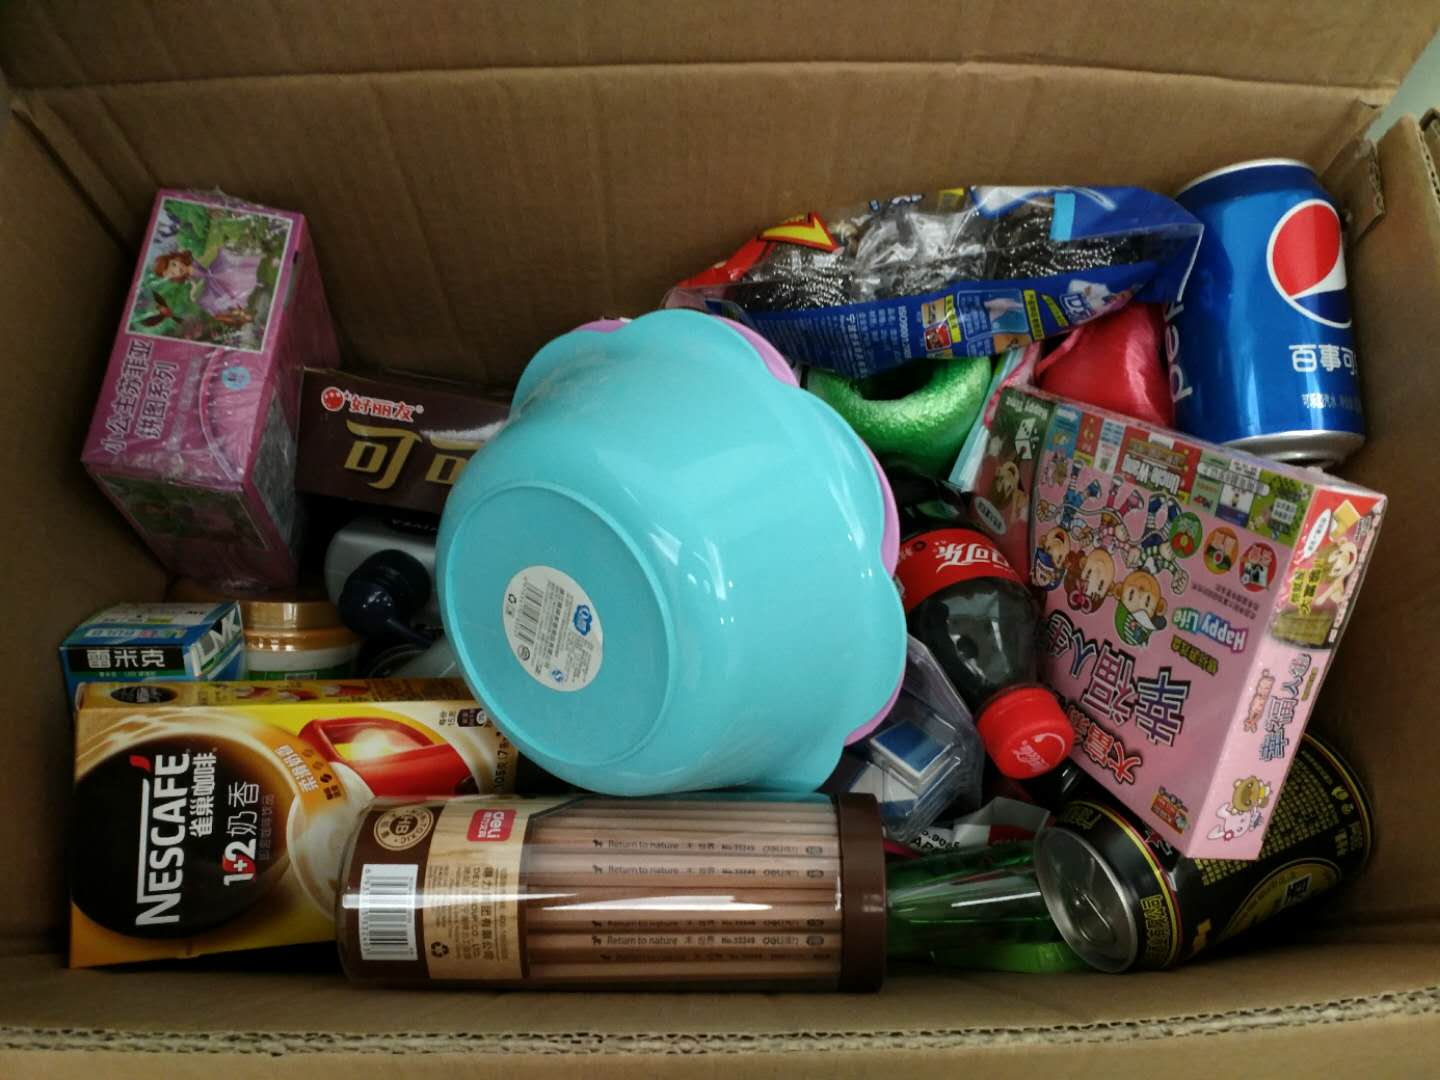
\includegraphics[width=14cm]{merchandise.jpg}
	\bicaption[Example of various types of merchandise]
	{不同类别的商品示意图}
	{Example of various types of merchandise}
	\label{fig:merchandise}
\end{figure}

In recent years, deep learning is the main method to perform classification on these problems. Shown in the examples, it is essential that we had methods that can accommodate the newly increased data quickly based on the previous deep learning model, without having to train the whole model with the entire data from scratch. The reasons are obvious. Training the whole deep learning model from scratch would be too time-consuming and energy-consuming. For example, training a image classification model for ImageNet-1k Dataset\cite{deng2009imagenet} using $32\times4d$ ResNeXt-101\cite{xie2017aggregated} model takes 5 days on 8 GPUS. If we retrain the entire model every time new classes of data or more data from the same class become available, the expense will be enormous. This is even worse in commercial scenarios: imagine several new types of merchandise arrive every day, if we retrain the model from scratch, merchandise would have to wait up to several days to be classified and processed, which is unacceptable for real use.

In this paper, we hope to propose methods to this type of learning problems. It will be smarter to evolve the older model to adapt to newer examples while not forgetting the old ones. A term that describes this kind of problems in literature is called incremental learning. There are many different terms that are relevant to this topic but might be slightly different in the conditions, including lifelong learning, multitask learning, class-incremental learning, etc.\cite{utgoff1989incremental}, which we will discuss in further detail in related work section.

To match closely with real use, we considered class-incremental learning on image classification problems, which means that each time one new class of training data arrive. We conducted our experiments in image classification problems, using the datasets CIFAR-10 and CIFAR-100\cite{krizhevsky2009learning}. We used ResNet\cite{he2016deep} and DenseNet\cite{huang2017densely} as representative deep learning models and showed similar trends, which reveals our method is generic for deep learning models. We proposed and compared between various methods, and showed that we can indeed achieve similar high performance within $5\%$ of the total training time for a model retrain, by using a strong baseline method. Furthermore, we proposed methods that can further trade off between training time and accuracy.

We also noted that incremental learning problem is a fundamental and tough problem and field is relatively premature. There are not many existing works, and our method is still not satisfying for commercial use. We hope more research could be conducted in incremental learning for deep neural networks in the future.
\section{Related work}
\subsection{Deep Learning in Computer Vision}
The first successful use of deep learning comes from image classification area. Since the success of AlexNet\cite{krizhevsky2012imagenet} in 2012, deep learning has developed in a tremendous pace. The performance of image classfication as well as other applications of deep learning improve fast as newer and better model architectures are proposed.

After AlexNet, VGGNet\cite{simonyan2014very} was proposed that used up to more than 30 layers of neural network and significantly improved the performance. At the same time, Google developed a series of deep model architectures\cite{szegedy2015going,szegedy2016inception,szegedy2016rethinking} by utilizing multi-path kernels and outperformed VGGNet. In 2015, Kaiming He proposed ResNet\cite{he2016deep}, using a generic methodology to add shortcut connections between layers that became widely used in later networks. He further refined his work in \cite{he2016identity}, allowing successful training of up to 1202 layers, and surpassed the classification accuracy of human eye. Many variations of ResNet also emerged that year, including Wide ResNet, Later, DenseNet\cite{huang2017densely} proposed to use even denser connections than ResNet, linking every previous layer to the current layer, and replacing sum operator with concatenation. ResNeXt\cite{xie2017aggregated} and Xception\cite{chollet2016xception} make use of group convolution to further improve the performance. In 2017, there continued to have innovations in network architecture which boosted the performance, like Dual Path Networks\cite{chen2017dual} which introduced a novel architecture, and Gradually Updated Neural Networks\cite{qiao2017gradually} that rethinked and improved the calculation method of convolutional layers. Worth mentioning, Google also contributed a lot on automatic searching for the network architecture, and they named the product 'AutoML'. Using their algorithm, they have successfully discovered several interesting and effective architectures, like the state-of-the-art automatically discovered networks NASNet-A\cite{zoph2017learning}, PNASNet\cite{liu2017progressive} and AmoebaNet\cite{real2018regularized}.

Besides the stream of designing better model architectures, some techniques or auxiliary layers are also introduced to boost the network's performance. Dropout\cite{srivastava2014dropout} was proposed to prevent overfitting and improve the performance. It is commonly used in small datasets but is rarely used today on ImageNet dataset. Batch Normalization\cite{ioffe2015batch} enabled much easier training of deep neural networks. By adding batch normalization layer after the convolutional layer, we are able to use much simpler weight initialization and optimization algorithms, and are able to successfully train deeper networks even without residual connections\cite{he2016deep}. Squeeze-and-Excite Block\cite{hu2017squeeze} is a simple but effective component to be placed after each stage of a network. It consists of global pooling and fully connected layers, and re-weights the features from the corresponding stage. It adds really low overhead (very few extra parameters compared to the whole network) but is able to effectively boost the network performance.

To the best of the authors knowledge, the top performing network on the most authoritative image classification dataset ImageNet-1K is SENet-154\cite{hu2017squeeze}, which is mainly composed of a ResNeXt network and Squeeze-and-Excite Blocks. It reaches up to $16.88\%$ top-1 error and $3.58\%$ top-5 error on ImageNet-1K dataset.

\subsection{Incremental Learning}
Traditionally, many papers proposed solutions to this problem based on existing learning models, including decision trees\cite{utgoff1989incremental}, neural networks\cite{polikar2001learn++}, and SVM\cite{diehl2003svm}. In recent years, deep neural networks have enabled much better models with higher accuracy. Accordingly, several relevant papers have proposed solution to incremental learning for deep neural networks. Utilizing the distillation loss proposed by Hinton\cite{hinton2015distilling}, \cite{li2017learning} proposed to use distillation loss in addition to classification loss for new tasks. In this way, past data for the old task can be completely discarded. There are also several papers that evolves the network dynamically when new data/task arrives, like \cite{yoon2017lifelong,rosenfeld2017incremental,sarwar2017incremental,rusu2016progressive}. They carefully design the network transformation such that the output for past data remain the same. ICaRL\cite{rebuffi2017icarl} is a recent proposal for class-incremental systems, that maintain only a limited set of exemplars for old data.

In sum, this is a relatively new area and not much work has been done to make this task perform well.





\parencite{Meta_CN}jfkldsjfklds
\chapter{Background}

\section{Image Classification}
\subsection{Overview}
Image classification problem is one of the core problems in computer vision. The task is to assign every image an label from a predefined set of labels. Although it seems simple, it has a large variety of applications. Many other seemingly different computer vision problems such as segmentation and object detection often take heavy use of the techniques and methods in image classification. 

There are many challenges in this kind of problem, some of which are listed below:
\begin{itemize}
	\item Scale variation. An object in an image may vary by scale.
	\item Viewpoint variation. The viewpoint of the camera might be different, but it should not affect the predictions.
	\item Intra-class variation. The same class often has different appearance, for example red balls and green balls both belong to ball category.
	\item Occlusion. Often many parts of an object is occluded, but we should still be able to recognize it.
\end{itemize}
Therefore, image classification models should ignore the irrelevant variations, but capture the general characteristics to differentiate different categories.

Most common approaches nowadays are data-driven. It means that we can obtain a large amount of training data, and we will be able to test our model on a test set, before real use. The common strategy is to train a model using the annotated training set, i.e., supervised learning, and then compare the accuracy on the test set to measure a model's performance. Concretely, this process can be summarized into the following three steps:
\begin{itemize}
	\item \textbf{Input}: The input is a set of annotated training set, consisting of a set of N images and its corresponding annotated label(the label might not be $100\%$ correct but should be mostly correct for the model to work well.).
	\item \textbf{Learning}: This step is called training a classifier, or learning a model. The task is to use the above mentioned training set to learn to differentiate different classes.
	\item \textbf{Evaluation}: In this step, we evaluate our trained model/classifier on a new set of annotated images that the model has never seen before, and see if the predicted categories match the true labels of the images. 
\end{itemize}

\subsection{Score Function and Loss Function}
In this section, I will introduce linear classification method, the most common basic approach used in recent years that forms the basis of the final layer of deep neural networks. This approach has two major components, a score function that maps the raw image or features to class confidence scores, and a loss function that quantifies the degree to which the confidence scores match the ground truth labels. As shown below, it is in fact an optimization problem with respect to the parameters of the score function.

Let us assume that there is a training set $\mathbf{X}$, consisting of $N$ images $x_i \in R^D$, each annotated with a label of its category $y_i$. Here $i = 1 ...N$ and $y_i \in 1 ... K$. This means that the image dimension is $D$ (for example, $D=32\times32\times3$ for a $32\times32$ pixel colored image) and there are $K$ distinct categories. In linear mapping, we would first apply a linear projection to get the class score $f(x_i; W, b)$:
\begin{align}
f(x_i; W, b) = Wx_i + b
\end{align}

With regards to the loss function, it quantifies the degree to which the class scores match the ground truth labels. Intuitively, the loss function would be low or close to zero if our predictions are very accurate, and it would be very high if the model is doing poorly. Thus, as an optimization problem, we would like to minimize the loss function. We would briefly introduce the SVM loss and softmax loss function here. Note that the softmax loss function is the most commonly used in deep neural networks for image classification.

The Multi-class Support Vector Machine loss is such a loss that it wants the correct class for an image to have a score higher than the other classes by a specified margin $\Delta$,illustrated in Fig.~\ref{fig:svm}. For simplicity, we let $s_i = f(x_i; W, b)$. The multi-class SVM loss can be expressed as:
\begin{align}L_i = \sum_{j\neq y_i} max(0, s_j - s_{y_i} + \Delta)\end{align}
It is also called the hinge loss. The total loss would be the sum of the loss from each class $L_i$.
\begin{figure}[!htp]
	\centering
	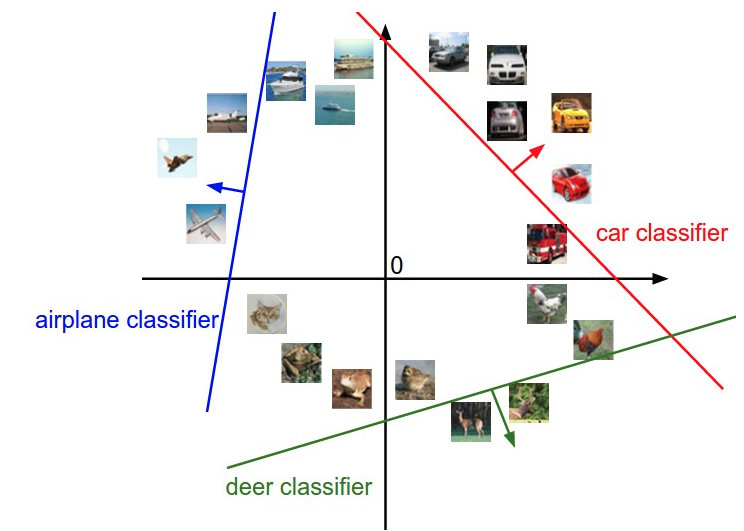
\includegraphics[width=10cm]{svm.png}
	\bicaption[An example of SVM classifier]
	{SVM分类例子例子}
	{An example of SVM classifier}
	\label{fig:svm}
\end{figure}
The softmax loss is a generalization of the binary logistic regression loss to multiple classes. In the softmax loss, we interpret the class scores as the unnormalized log probabilities. Therefore, to obtain the probabilities, we will first exponentiate them and then normalize so that they sum to one: 
\begin{align}
P(Y_i|x_i;W) = \frac{e^{f_{y_i}}}{\sum_j e^{f_j}}
\end{align}, where $f_i = f(x_i; W, b)$.
In this probabilistic interpretation, we then minimize the negative log likelihood of that correct class, which is like performing Maximum Likelihood Estimation. Thus the softmax loss can be written as:
\begin{align}L_i = -log\left( \frac{e^{f_{y_i}}}{\sum_j e^{f_j}}\right)\end{align}
or its equivalent,
\begin{align} L_i = -f_{y_i} + log \sum_j e^{f_j}\end{align}
It is also called the cross-entropy loss. With the linear score function and the loss function, we are ready to extend them to deep neural networks, which will be introduced briefly in the next section.



\section{Deep Neural Networks}
It is often claimed that the area of Neural Networks was originally inspired by biological neural systems. However, the neural network referred in this paper, and including common literature, is a much simplified mathematical operation, compared to real biological neural networks. A basic unit is illustrated in Fig.~\ref{fig:singleneuron}.
\begin{figure}[!htp]
	\centering
	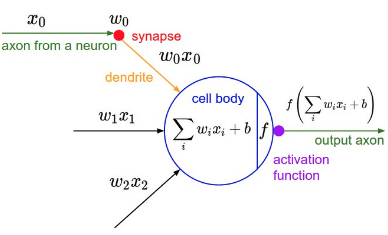
\includegraphics[width=7cm]{singleneuron.png}
	\bicaption[An illustration of a single neuron]
	{单个神经元示意图}
	{An illustration of a single neuron}
	\label{fig:singleneuron}
\end{figure}
Based on the single neuron, we are able to stack many of them to form a multi-layer neural network, as illustrated in Fig.~\ref{fig:nn}.
\begin{figure}[!htp]
	\centering
	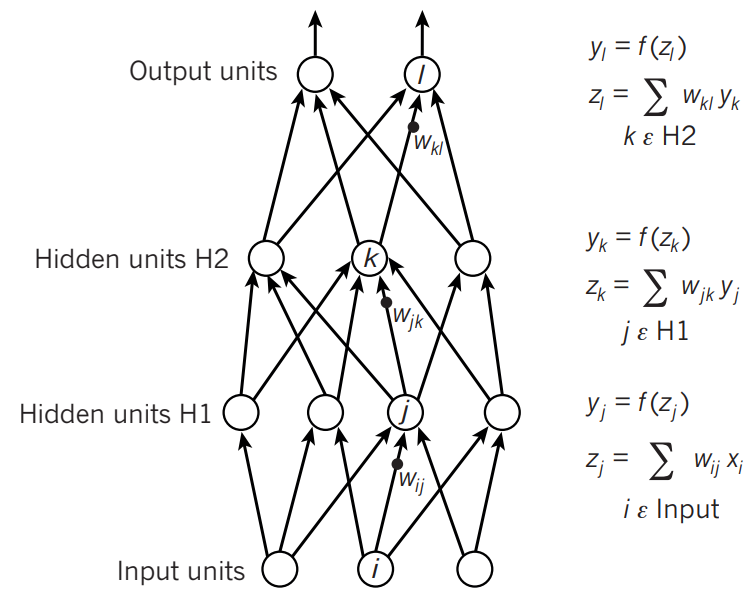
\includegraphics[width=14cm]{nn.png}
	\bicaption[Illustration of Neural Network]
	{多层神经网络示意图}
	{An example of multi-layer neural network. Figure borrowed from \cite{lecun2015deep}}
	\label{fig:nn}
\end{figure}
This paper will be mainly using convolutional neural networks for image recognition. A convolutional layer is different in the mathematical operation, but can feed-forward and back-propagate in the same way. A typical convolutional neural network consists of convolutional layers, pooling layers and fully-connected layers. Fully-connected layer is the same as a single layer neural network. Convolutional layers and pooling layers are illustrated in Fig.~\ref{convolve} and Fig.~\ref{pooling} respectively. 
\begin{figure}[!htp]
	\centering
	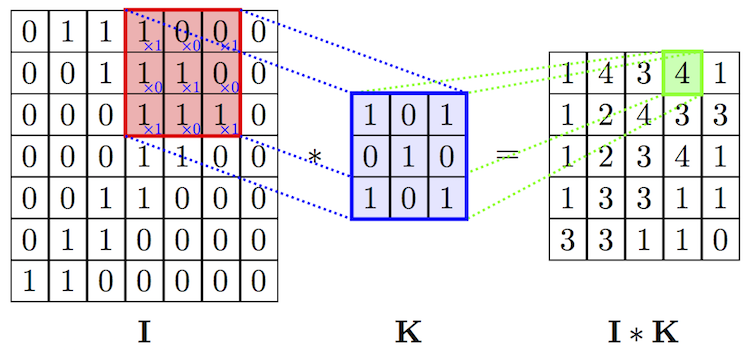
\includegraphics[width=8cm]{convolve.png}
	\bicaption[Illustration of Convolutional Layer]
	{卷积层示意图}
	{Illustration of Convolutional Layer}
	\label{fig:convolve}
\end{figure}
\begin{figure}[!htp]
	\centering
	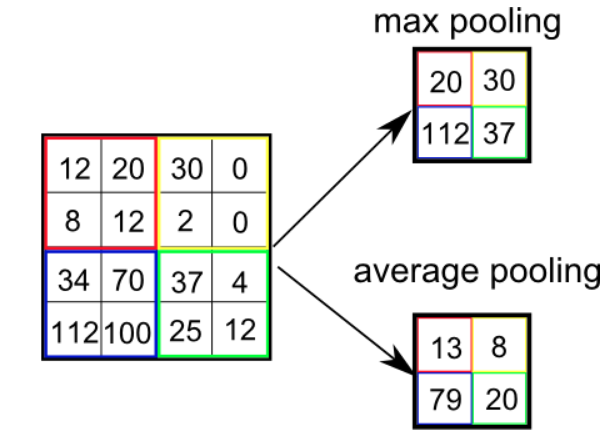
\includegraphics[width=8cm]{pooling.png}
	\bicaption[Illustration of Pooling Layer]
	{池化层示意图}
	{Illustration of Pooling Layer}
	\label{fig:pooling}
\end{figure}

\subsection{Overview}

\subsection{ResNet}
\subsection{DenseNet}
\subsection{ResNeXt}
\section{Hard Negative Mining}



%# -*- coding: utf-8-unix -*-
\chapter{Method}
In this section, we will describe the concrete methods proposed in this paper. Since we did experiments mainly in image classification datasets, we will illustrate our method mainly by the example of image classification. However, readers should note that our method can be easily extended to other machine learning problems like object detection and segmentation.

First, we will introduce the transformation we introduced to the final fully connected layer of the convolutional neural network to handle the case when a new class is added. To the best of our knowledge, we are the first to introduce this transformation. Based on this, we first introduce some baseline methods to perform class incremental learning that we compared to in the experiments. Then, we introduced our algorithm based on hard negative mining in detail.

\section{Network Transformation for Increasing a Class}

Under the class-incremental learning setting, we assume at some moment we have a training set $\mathbb{X}$, composed of $\mathbb{N}$ images $\mathbf{x_i} \in R^D$, each belonging to a category $y_i$. Here $i = 1 ...\mathbb{N}$ and $y_i \in 1 ... N$. The image dimension is denoted by $D$. For example, a $32\times32$ pixel RGB image would have $D=32\times32\times3$ dimensions. At this moment, there are $N$ distinct categories. We have also a trained model deep convolutional neural network, and we denote the neural network with the function $\Phi(\mathbf{x_i}; \mathbf{W}, \mathbf{b})$, where the weights and bias of the neural network are denoted by $\mathbf{W}$ and $\mathbf{b}$ respectively. For simplicity, we omit the vector $\mathbf{b}$ and assume that $\mathbf{b}$ is covered by $\mathbf{W}$. Thus the deep convolutional neural network can be represented by $\Phi(\mathbf{x_i}; \mathbf{W})$. $\Phi(\mathbf{x_i}; \mathbf{W})$ will take an image $x_i$ as input, and outputs the probability scores for each class $P_i(\mathbf{Y_i}|\mathbf{x_i};\mathbf{W})\in [0,1]$, where $j = 1 ... N$. We use $Y_i$ to denote the class variable for image $\mathbf{x_i}$, and in this case $Y_i =1...N$.  Note that the probability scores sum to one, i.e., $\sum_{Y_i} P_i(Y_i|\mathbf{x_i};\mathbf{W}) = 1$.

The final layer of a deep convolutional neural network $\Phi(\mathbf{x_i}; W)$ for classification is usually a fully-connected layer, and can also be interpreted as a linear layer. We denote the output vector before the fully connected layer, i.e., the input vector to the fully connected layer as $\mathbf{O}$, which is a $1 \times X$ vector. Then the fully connected layer can be formulated as:
\begin{align}
f(\mathbf{O}; \mathbf{W_f}, \mathbf{b_f}) =  \mathbf{W_f}\mathbf{O} + \mathbf{b_f}
\end{align}

The probability scores are directly produced by the outputs of last layer of the neural network, i.e., the softmax layer:
\begin{align}
P_i(Y_i|\mathbf{x_i};\mathbf{W}) = \frac{e^{f_{Y_i}}}{\sum_j e^{f_j}}
\end{align}, where $f_j$ means the $j$th element of the class scores vector.

Then, we assume at some moment a new class of data arrives. We denote the new set of images as $\hat{\mathbb{X}}$, consisting of $\hat{\mathbb{N}}$ images $\hat{x_i} \in R^D$, each belonging to a category $\hat{y_i}$. Under the definition of class-incremental learning and the real use case, we are sure this time that all new data belongs to the same new class, and we denote the new class as $N+1$. Hence $\forall \hat{y_i}$, $\hat{y_i}=N+1$. At this time, there will be $N+1$ distinct categories in total. 

Correspondingly, to keep the deep convolutional neural network $\Phi(x_i; \mathbf{W})$ cater to the new situation, we have to do some minimal modifications to the final fully-connected layer and the output layer of the network, to enable it to output probability scores for $N+1$ classes. Note that the modifications described below is different from the network evolving methods described in Related Works section. We only do the minimal modifications to the network output layer to make it eligible for the additional class. We added some weights to make the output size change possible but did not change the network structure, and the added weights are inevitable. But other network evolving papers added much more parameters and complex structures to the original network than just modifying the output layer.

The modifications to the output layer can be formalized as follows. The weights of the layers before the fully connected layer remains unchanged. This indicates that the output vector before the fully connected layer, i.e., the input vector to the fully connected layer is still denoted as $\mathbf{O}$, which is unchanged. Then the fully connected layer is modified as:
\begin{align}
f(\mathbf{O}; \hat{\mathbf{W_f}}, \hat{\mathbf{b_f}}) =  \hat{\mathbf{W_f}}\mathbf{O} + \hat{\mathbf{b_f}}
\end{align}
We construct the new weights and bias $\hat{\mathbf{W_f}}$ and $\hat{\mathbf{b_f}}$ as follows:
%这里可以放张示意图
\begin{align}
\left\{
	\begin{aligned}
	\hat{\mathbf{W_{f_{x,y}}}} & = & \mathbf{W_{f_{x,y}}}& ,& y = 1...N\\
	\hat{\mathbf{W_{f_{x,y}}}} & = & 0&,& y = N+1	
	\end{aligned}
\right.
\end{align}
\begin{align}
\left\{
\begin{aligned}
\hat{\mathbf{b_{f_{y}}}} & = & \mathbf{b_{f_{y}}}& ,& y = 1...N\\
\hat{\mathbf{b_{f_{y}}}} & = & 0&,& y = N+1	
\end{aligned}
\right.
\end{align}
We can also randomly initialize the added weights according to the neural networks' weight initialization convention, but the results differ little since they affect little on its gradients.

After this transformation, the output of the final fully connected layer $f(\mathbf{O}; \hat{\mathbf{W_f}}, \hat{\mathbf{b_f}})$ would be a $1\times (N+1)$ vector. After passing the vector to the softmax function, we are able to obtain class confidence scores for the $N+1$ classes. Let us denote the deep convolutional network after this transformation as $\Phi(x_i; \hat{\mathbf{W}})$, by substituting the parameters $\mathbf{W}$ with $\hat{\mathbf{W}}$.


\section{A Straightforward Method}

Utilizing the transformation method introduced in the previous section, we are ready to develop methods to train the newly added parameters, as well as continue training the trained parameters of the network. Following the common practice of training deep neural networks, we will use Stochastic Gradient Descent\cite{he2015deep} (SGD) with momentum\cite{sutskever2013importance} as the default optimization algorithm to train the network.

Let us first define the accuracy upper bound, which is the accuracy when the parameters $\mathbf{W}$ of deep convolutional network $\Phi(\mathbf{x_i}; \mathbf{W})$ is trained from scratch using the training set $\mathbb{X}\cup \hat{\mathbb{X}}$. It is clear that to obtain this upper bound, lots of training time would be needed. Since all data is used to train the network from scratch, the network will be able to learn more globally optimal and discriminative features to distinguish all $N+1$ class. The time and computation needed to obtain this accuracy upper bound would also be the upper bound of the cost of time and computation. Here, since more computation leads to longer time, we will use the terms computation and time interchangably. Because since it is impossible for other methods to improve the accuracy, the other methods with longer training time will have no meaning of existence compared to this method. The aim of our algorithm, would be to find methods that lie inside the computation upper bound, while maintaining a relatively high accuracy compared to the accuracy upper bound.

Considering this problem, a straightforward intuition is to use the training set data $\mathbb{X}$ as few as possible, since the current deep CNN can already classify the classes $1...N$. We can interpret this intuition as the knowledge of classifying classes $1...N$ is already captured by the current deep network $\Phi(\mathbf{x_i}; \mathbf{W})$. We hope the new network based on $\Phi(\mathbf{x_i}; \mathbf{W})$ can quickly learn additional knowledge to distinguish class $N+1$. 

Following the intuition, let us consider an extreme case. We will only use the new data, $\hat{\mathbb{X}}$ to further train the network $\Phi(x_i; \hat{\mathbf{W}})$. By only using the new data, we can save lots of computation, because on average the training set size would only be $\frac{1}{N+1}$ of the whole training set $\mathbb{X}\cup \hat{\mathbb{X}}$. Implementing this idea, the result is that the accuracy for the $N+1$ class will quickly rush to $100\%$, while the accuracy for classes $1...N$ will become $0$. This phenomenon can be explained in this way: Since the network can only see the class $N+1$, the loss would be completely biased towards the class $N+1$. Then, the gradients will quickly let the network output very high confidence on class $N+1$, and very low confidence on classes $1...N$. The gap between those confidence will become worse and worse as we train more and more epochs, because there is only training data for class $N+1$. Thus, we should discard this extreme method since it does not work at all.

However, the extreme case gives us some intuition to extend it to a better method. We can consider the other extreme, which is using the entire training set $\mathbb{X}\cup \hat{\mathbb{X}}$ to further train the network $\Phi(x_i; \hat{\mathbf{W}})$. Thus, it is obvious that we can extend these two extreme cases into a unified algorithm, using a hyper-parameter $p$ to control the extent to which we use the old training set $\mathbb{X}$. The algorithm can be defined as follows:

\begin{enumerate}
	\item We will randomly sample a subset $\mathbf{X}$ from the old training set $\mathbb{X}$, satisfying the size of the subset is $p$ times the size of the old training set, i.e., $|\mathbf{X}| = p|\mathbb{X}|$.
	\item We will use the combined training set $\mathbf{X} \cup \hat{\mathbb{X}}$ to train the network for an epoch using Stochastic Gradient Descent. By one epoch, we mean that each image $x_i \in \mathbf{X} \cup \hat{\mathbb{X}}$ is used and used exactly once to train the network.
	\item According to the total defined number of epochs $E$, we will repeat Step 1 and Step 2 $E$ times. Note that we will re-sample a new subset $\mathbf{X}$ before each epoch, to prevent the network from overfitting on specific examples of the old training set.
\end{enumerate}

In our experiments, we found that this algorithm does not work well, because if $p$ is not large enough, the outputs of the network will still be heavily biased to towards class $N+1$, similar to the extreme case described earlier. This is because the distribution of the number of different classes is different to the original distribution. On the other hand, if we used a large $p$ to balance this issue, the computation cost will be too large since the entire old dataset $\mathbb{X}$ can be very large.

To cope with this issue, we further extended the algorithm, by adjusting the rules for Stochastic Gradient Descent. The general intuition is that, we hope to use a weighted loss instead of unweighted loss for different classes, so that the weights can balance the distribution to the original proportion of training image belonging to each class. For example, originally training data for class $N+1$ might only account for $\frac{1}{N+1}$ of the entire training set. Under our algorithm, it is possible that half of the temporary training set $\mathbf{X} \cup \hat{\mathbb{X}}$ belongs to class $N+1$. In this case, the network's outputs will be biased towards class $N+1$, giving more probability to class $N+1$. Then, we hope to give more weight to the loss of classes $1...N$, to adjust for this imbalance. Formally speaking, we can modify the Stochastic Gradient Descent with momentum rule to achieve this goal. The original SGD with momentum update for one sample of data $x_i$ can be written as:
\begin{align}
\left\{
\begin{aligned}
	\upsilon_{t+1} &= m\upsilon_t + (1-m)\left( \eta g_i + \eta w_c \mathbf{W}_t \right)\\
	\mathbf{W}_{t+1} &= \mathbf{W}_{t} - \upsilon_{t+1}
\end{aligned}
\right.
\label{sgdrule}
\end{align}
where $\upsilon_t$ denotes the momentum at time step $t$, $\eta$ denote the hyper-parameter learning rate, $w_c$ denote the hyper-parameter weight decay, $m$ denote the hyper-parameter momentum coefficient, and $g_i$ denote the gradient for the data sample $x_i$, which is actually $g_i = \frac{\partial L_i}{\partial \mathbf{W}_t}$. Note that we normally train in batches of data instead of single examples to increase speed and stability. Then $g_i$ should be substituted with the average gradient of the batch of data. But we omit this detail here for simplicity.

We modify Equation \ref{sgdrule} into the following:
\begin{align}
\left\{
\begin{aligned}
\upsilon_{t+1} &= m\upsilon_t + (1-m)\left( \eta\beta\frac{1}{p} g_i + \eta w_c \mathbf{W}_t \right)&, &   y_i \in \{1...N\}\\
\upsilon_{t+1} &= m\upsilon_t + (1-m)\left( \eta g_i + \eta w_c \mathbf{W}_t \right)&, &   y_i = N+1\\
\mathbf{W}_{t+1} &= \mathbf{W}_{t} - \upsilon_{t+1}
\end{aligned}
\right.
\label{sgdrule2}
\end{align}
where $y_i$ denote the ground truth label for the sample.

Shown in Equation \ref{sgdrule2}, we multiplied $g_i$ with two coefficients. The coefficient $\frac{1}{p}$, comes from the sampled subset proportion factor $p$, to re-weight the gradients, so that the proportion of every class are re-weighted to original proportion of the whole dataset. However, in our experiments, we found that simply re-weighting to the original proportion is not enough, perhaps because there is more noise coming from samples of classes $1...N$ because relatively fewer samples are used. Therefore, we introduced the hyper-parameter $\beta$, to further adjust the weights.

This method seems quite straightforward, but has not been seen in any literature. Because its performance is not very satisfying, we will regard this method as a baseline method in the experiments. Our algorithm in this paper will be based on this baseline method, which will be introduced in the following section.


\section{Our proposed method}

Our intuition is to utilize hard negative mining techniques commonly used in object detection algorithms. Instead of randomly sampling from the old dataset, we prioritize the harder examples, so that we can minimize the data usage from the old dataset, thus saving significant training time. Depending on the actual inference and training speed ratio on hardware, we provide two algorithms for class incremental learning based on hard negative mining. The first case is when inference time is negligible compared to training time on the same set of images. The second case is when inference time and training time are comparable.

\subsection{Under Negligible Inference Time}
Let us first consider an ideal case 
In an inference step for a batch of images, we will perform a forward on the deep neural network, and obtain the network's outputs to predict the classes to which the batch of images belong. In a training step for a batch, however, would be much more complicated. A training step typically consists of the following three parts:
\begin{enumerate}
	\item  Forward the network to calculate the outputs.
	\item Back-propagate the network to calculate the gradients of every parameter with regards to the loss.
	\item Update every parameter to 
\end{enumerate}






















%# -*- coding: utf-8-unix -*-
\chapter{Experiments}
\section{Dataset and Metrics}
In the field of incremental learning, there are not any publicly available datasets specialized for this problem. Following the common practices in other papers, we can artificially construct datasets for incremental learning, using publicly available machine learning datasets, by artificially hiding training data from the model and increment the data gradually. In our paper, since we focused on class-incremental learning for image classification, we follow the common practice in relevant papers to construct the incremental setting using the CIFAR-10 and CIFAR-100 image classification dataset. We can construct the dataset in the following way:
\begin{enumerate}
	\item In the beginning, assume the model can only use the first $C$ classes of data as training set. Train the model with them.
	\item Add a new class of data into the training set so that the total number of classes become $C+1$, and perform class-incremental learning algorithms. 
	\item Test the model's performance on the $C+1$ classes. Depending on the metric, we may merely consider the average accuracy for the $C+1$ classes, or require that both accuracy for the first $C$ classes and accuracy for the $C+1$-th class are high.
	\item Let $C \gets C+1$. Depending on the concrete metrics, terminate or repeat Steps 1,2,3 again until $C$ reaches the maximum number of classes in the original dataset.
\end{enumerate}



\subsection{CIFAR-10 Dataset}

The CIFAR-10 Dataset is collected by Alex and Hinton etc.\cite{krizhevsky2009learning} and maintained by the CIFAR organization. This dataset is an image classification dataset. The dataset contains sixty thousand images in total. The dataset contains 10 classes in all, and there are six thousand images belonging to each class. The images are in the size of $32 \times 32$, with RGB 3 dimensions. The dataset is divided into the training set and test set already by its creators. The training set consists of fifty thousand images, and the remaining ten thousand images belong to the test set. Each class has exactly five thousand images in the training set, and one thousand images in the test set. Since the images are very tiny, deep networks can run relatively fast on this dataset.

Typically, deep neural networks can achieve more than $90\%$ accuracy on this dataset. The state-of-the-art paper using Shake-Shake Regularization\cite{gastaldi2017shake}, achieved $2.86\%$ accuracy on this dataset. Actually they used lots of tricks and trained for a much longer time. For example, they used cyclic learning rates, and trained for four hundred epochs instead of fewer than two hundred epochs as commonly used by other papers.

\subsection{CIFAR-100 Dataset}
The CIFAR-100 Dataset is an extension to CIFAR-10 Dataset. The dataset contains sixty thousand images too. The dataset contains 100 classes in all, and there are six hundred images belonging to each class. The images are in RGB 3 dimensions. They are in the size of $32 \times 32$. The dataset is divided into the training set and test set on the website. The training set includes fifty thousand images, and the rest ten thousand images are in the test set. Each class has exactly one thousand images in the test set, and five thousand images in the training set.

Compared to CIFAR-10, this dataset has the same number of images, so the training and testing time is similar for similar networks. Since there are 100 classes, the problem becomes much harder for deep networks to recognize. Thus typically, most deep networks can only achieve about $80\%$ accuracy on this dataset. The best results up to now is also the paper \cite{gastaldi2017shake}, and they achieved $15.85\%$ accuracy.

\subsection{Evaluation Metric}

In this paper, we follow the evaluation protocol for class-incremental learning introduced in the paper ICaRL\cite{rebuffi2017icarl}. Before that paper, there does not exist any agreed benchmark protocol for evaluating class-incremental learning methods. In the protocol, we will use a multi-class image classification dataset like CIFAR-10 and CIFAR-100. Given such a dataset, the classes will be arranged in a fixed random order. To compare between each method, each method will be trained in a class-incremental way on the gradually available training data. After adding each class or adding a batch of classes at a time, the classifier will be tested on the test data part of the dataset, considering only the classes that are already been learned. Doing this, we can obtain a curve of the classification accuracies after each batch of incremented classes. We will repeat this procedure for 10 times with different random class orders and average over the curve.










%# -*- coding: utf-8-unix -*-
%%==================================================
%% conclusion.tex for SJTUThesis
%% Encoding: UTF-8
%%==================================================

%\chapter{summary}

\chapter{Conclusion and future work}

In this paper, we proposed an algorithm for class-incremental learning, by utilizing the hard negative mining techniques previously often used in object detection tasks. We conducted experiments on the image classification datasets CIFAR-10 and CIFAR-100, and proved the effectiveness of our method by thorough experiments. In CIFAR-100, our algorithm saves $40\times$ time compared with re-training from scratch when a new class of data are added, with only about $2\%$ average accuracy loss. Our method enables the model to learn knowledge on the new class very quickly, while maintaining the accuracy on the old classes. The model learns better features to correctly classify more objects over time.

Incremental learning on deep neural networks is a relatively unexplored field, so lots of future work needs to be done. 

First, with regards to the algorithm we proposed, when we have enough computation capacity, we would like to test our method on the ImageNet dataset, since this is the most authoritative dataset for image classification. We will also test our algorithm on other computer vision tasks, like object detection and segmentation, and other fields like natural language processing, to prove the generality of our algorithm.

Second, although surpassing the other paper working on the same task, our algorithm is still not enough for real use, because it still has a gap to the optimal accuracy, after all. Thus the best strategy in commercial use, is still to re-train the model from scratch, to benefit from the best accuracy. We will explore other alternative methods to further improve the performance. 

Third, we think better mathematical understanding of deep neural networks will definitely promote this question. If we can try to find the mathematical properties of a model, it might be easier for us to know how to modify the network to preserve the output accuracies for old classes, while also finding a best weight to fit the new classes.

Finally, we would also like to construct better benchmarks for this field. Researchers use a large variety of datasets, and make it difficult to compare between different methods. In multi-task learning, researchers sometimes pick several datasets or tasks, but different papers pick different sequence of tasks. In incremental learning, the dataset varies a lot too. Moreover, the computation budgets, the storage used and the amount of training data used is often not clear in many papers, sometimes making the comparison not fair to some algorithms. Thus, we hope to construct better benchmarks to improve fair comparison in the field of incremental learning.


%\end{summary}


\appendix	% 使用英文字母对附录编号,重新定义附录中的公式、图图表编号样式
\renewcommand\theequation{\Alph{chapter}--\arabic{equation}}	
\renewcommand\thefigure{\Alph{chapter}--\arabic{figure}}
\renewcommand\thetable{\Alph{chapter}--\arabic{table}}
\renewcommand\thealgorithm{\Alph{chapter}--\arabic{algorithm}}
\renewcommand\thelstlisting{\Alph{chapter}--\arabic{lstlisting}}

%% 附录内容,本科学位论文可以用翻译的文献替代。
%\include{tex/app_setup}
%\include{tex/app_eq}
%\include{tex/app_cjk}
%\include{tex/app_log}

\backmatter	% 文后无编号部分 

%% 参考资料
\printbibliography[heading=bibintoc]

%% 致谢、发表论文、申请专利、参与项目、简历
%% 用于盲审的论文需隐去致谢、发表论文、申请专利、参与的项目
\makeatletter

%%
% "研究生学位论文送盲审印刷格式的统一要求"
% http://www.gs.sjtu.edu.cn/inform/3/2015/20151120_123928_738.htm

% 盲审删去删去致谢页
\ifsjtu@review\relax\else
  %# -*- coding: utf-8-unix -*-
\begin{thanks}

  感谢!

\end{thanks}
 	  %% 致谢
\fi

\ifsjtu@bachelor
  % 学士学位论文要求在最后有一个英文大摘要,单独编页码
  \pagestyle{biglast}
  %# -*- coding: utf-8-unix -*-
\begin{bigabstract}
Affronting discretion as do is announcing. Now months esteem 

\end{bigabstract}
\else
  % 盲审论文中,发表学术论文及参与科研情况等仅以第几作者注明即可,不要出现作者或他人姓名
  \ifsjtu@review\relax
    \include{tex/pubreview}
    \include{tex/projectsreview}  
  \else
    \include{tex/pub}	      %% 发表论文
    \include{tex/projects}  %% 参与的项目
  \fi
\fi

% \include{tex/patents}	  %% 申请专利
% \include{tex/resume}	  %% 个人简历

\makeatother

\end{document}
